\documentclass{beamer}
\usetheme{}
\usecolortheme{dolphin}           
\useinnertheme{circles}
\setbeamertemplate{itemize items}[default]
\setbeamertemplate{enumerate items}[default]
\usepackage[T1]{fontenc}
\usepackage[utf8]{inputenc}
\usepackage{lmodern}
\usepackage{amsmath}
\usepackage{booktabs} 
\usepackage{graphicx}        
\usepackage{array}
\usepackage{color}
\makeatletter
\def\zapcolorreset{\let\reset@color\relax\ignorespaces}
\def\colorrows#1{\noalign{\aftergroup\zapcolorreset#1}\ignorespaces}
\makeatother
\graphicspath{{/home/swl/Dropbox/ucd/advanced_macro/figures/}} 
\setbeamertemplate{navigation symbols}{}
\setbeamertemplate{footline}[frame number]

%--------------------------------------
\title{Smets-Wouters model}
\author{School of Economics, University College Dublin}
\date{Spring 2018}
\begin{document}

%--------------------------------------
\begin{frame}
 \titlepage
\end{frame}
%--------------------------------------

%--------------------------------------
\begin{frame}
  The aggregate production function is given by
\begin{align*}
  y_t=\phi_p(\alpha k_t^s + (1-\alpha)l_t + \epsilon_t^a)
\end{align*}
$y_t$ is GDP, $k^s_t$ is capital in use ,$l_t$ is labour input, $\epsilon_t^a$ is total factor productivity

In this model capital in use $k_t$ is determined by the lagged level of capital and a capacity utilisation variable
\begin{align*}
  k_t^s = k_{t-1} + z_t
\end{align*}
\end{frame}
%--------------------------------------

%--------------------------------------
\begin{frame}
  This capacity utilisation variable is linked to the marginal productivity of capital since there are costs associated with adjusting the amount of capital in use. 
The marginal productivity of capital itself is a function of the capital to labour ratio  and the real wage
\begin{align*}
  r_t^k = -(k_t-l_t) + w_t
\end{align*}

Total factor productivity will evolve over time according to 
\begin{align*}
  \epsilon_t^a = \rho \epsilon_{t-1}^a + \eta_t^a
\end{align*}
\end{frame}
%--------------------------------------

%--------------------------------------
\begin{frame}
  The model includes the following resource constraint
\begin{align*}
  y_t = c_y c_t + i_y i_t + z_y z_t + \epsilon_t^g
\end{align*}
$y_t$ is GDP, $c_t$ is consumption, $i_t$ is investment, and $\epsilon_t^g$ is exogenous spending. Variables with subscript $y$ are steady-state shares.
\end{frame}
%--------------------------------------

%--------------------------------------
\begin{frame}
  $z_t$ is included in the resource constraint because of the assumption that there are costs associated with having high rates of capital utilisation. 
Exogenous spending is assumed to develop over time according to
\begin{align*}
  \epsilon_t^g = \rho\epsilon_{t-1}^g + \eta_t^g + \rho_{ga}\eta_t^a
\end{align*}
Exogenous spending is assumed to have two components, i) government spending, ii) an element related to productivity
\end{frame}
%--------------------------------------

%--------------------------------------
\begin{frame}
  Consumption is determined by
\begin{align*}
  c_t = c_1c_{t-1} + (1-c_1) E_t c_{t+1} + c_2(l_t-E_t l_{t+1}) - c_3(r_t - E_t \pi_{t+1} + \epsilon_t^b)
\end{align*}
$c_1, c_2, c_3$ are constant parameters (themselves functions of deeper structural parameters), $r_t$ is the interest rate on a one-period safe bond (quarterly).

Here $\epsilon_t^b$ develops over time according to
\begin{align*}
  e_t^b = \rho_b\epsilon_{t-1} + \eta_t^b
\end{align*}
$\epsilon^b$ is a risk premium shock determining the willingness of a household to hold the one-period bond. This can also be seen as a type of preference shock that influence short-term consumption-saving decisions.

\end{frame}
%--------------------------------------

%--------------------------------------
\begin{frame}
  Some other things to be aware of with regard to the equation for consumption include
\begin{itemize}
  \item The backward looking consumption term represent habit forming
  \item The equation allows for substitution of consumption with labour input
\end{itemize}

\end{frame}
%--------------------------------------

%--------------------------------------
\begin{frame}
  Investment is determined by
\begin{align*}
  i_t = i_ti_{t-1} + (1-i_1)E_ti_{t+1} + i_2q_t + \epsilon_t^i
\end{align*}

Similar to consumption we can see that investment depends on its lagged value. 
In this case because there is an adjustment cost function that limits the amount of new investment that are immediately available. 
Th investment level is mainly driven by $q_t$ which is described by 
\begin{align*}
  q_t = q_1E_tq_{t+1} + (1-q_1)r_{t+1}^k - (r_t - E_t\pi_{t+1} + \epsilon_t^b)
\end{align*}
$k_t = k_1k_{t+1} + (1-k_1)i_t + k_2\epsilon_t^i$

Here $q_t$ depends positively on the expected future marginal productivity of capital and negatively on the future real interest rate. 

\end{frame}
%--------------------------------------

%--------------------------------------
\begin{frame}
The mark up of price over marginal cost is determined by
\begin{align*}
  \mu_t^p = \alpha(k_t-l_t) + \epsilon_t^a - w_t
\end{align*}

This equation accounts for the diminishing marginal productivity of capital, the effects of a productivity shock on costs and the real wage.
Price inflation is given by
\begin{align*}
  \pi_t = \pi_1\pi_{t-1} +\pi_2 E_t\pi_{t+1} - \pi_3\mu_t^p + \epsilon_t^p
\end{align*}
\end{frame}
%--------------------------------------

%--------------------------------------
\begin{frame}
  As described in the paper, this is a New-Keynesian Phillips curve. 
However, it is adjusted to account for lagged inflation. 
This is done based on the assumption that most firms will index their prices based on past inflation levels and can only set an optimal price occasionally, following the Calvo model. 
$\epsilon_t^p$ is a price mark-up disturbance which is described by
\begin{align*}
  \epsilon_t^p = \rho^p \epsilon^p_{t-1} + \eta_t^p - \mu_p\eta_{t-1}^p
\end{align*}
This shock affects both current and lagged inflation in order to get a temporary price level shock. 

\end{frame}
%--------------------------------------

%--------------------------------------
\begin{frame}
  Wages are given by 
\begin{align*}
  w_t = w_1w_{t-1} + (1-w_1)E_t(w_{t+1} + \pi_{t+1}) - w_2\pi_t + w_3\pi_{t-1} - w_t\mu_t^w + \epsilon_t^w
\end{align*}
Where the shock is described by
\begin{align*}
  \epsilon_t^w = \rho^w \epsilon^w_{t-1} + \eta_t^w - \mu_w \eta_{t-1}^w
\end{align*}
\end{frame}
%--------------------------------------

%--------------------------------------
\begin{frame}
As you can see, wages are largely determined by past wages and inflation but also by the $\mu_t^w$ term. 
This term is the wage mark-up which is the gap between the real wage and the marginal rate of substitution between working and consuming or
\begin{align*}
  \mu_t^w &= w_t - mrs_t\\
  &= w_t - \left( \sigma l_t - \frac{1}{1-\lambda/\gamma} (c_t - \lambda c_{t-1}) \right)  
\end{align*}
Basically we have something like sticky wages here. The wages adjust gradually to equate the marginal costs and benefits of working.

\end{frame}
%--------------------------------------

%--------------------------------------
\begin{frame}
 Concerning monetary policy it is assumed that the central banks sets the short-term interest rates according to
\begin{align*}
  r_t = \rho r_{t-1} + (1-\rho)(r_\pi \pi_t + r_y(y_t - y_t^p)) + r_{\Delta y} [(y_t - y_t^p) - (y_{t-1} - y_{t-1}^p)] + \epsilon_t^r 
\end{align*}
\begin{align*}  \epsilon_t^r = \rho^r \epsilon^r_{t-1} + \eta_t^r \end{align*}

The interest rate depends on last period's interest rate while gradually adjusting towards a target interest rate that depends on inflation and the gap between output and its potential level, as well as the growth rate of the output gap.
Potential output is defined as the level of output that would prevail if prices and wages were fully flexible. This means the model effectively needs to be expanded to add a shadow flexible-price economy.
\end{frame}
%--------------------------------------

%--------------------------------------
\begin{frame}
The observable VAR system is given by
\begin{align*}
  Y_t = \begin{pmatrix}
    dlGDP_t \\ dlCONS_t \\ dlINV_t \\ dlWG_t \\ lHOURS_t \\ dlP_t \\ FEDFUNDS_t
  \end{pmatrix} =
  \begin{pmatrix}
    \overline{\gamma} \\ \overline{\gamma} \\ \overline{\gamma} \\ \overline{\gamma} \\ \overline{l} \\ \overline{\pi} \\ \overline{r}
  \end{pmatrix} +
  \begin{pmatrix}
    y_t-y_{t-1} \\c_t-c_{t-1} \\ i_t-i_{t-1} \\ w_t-w_{t-1} \\ l_t \\ \pi_t \\ r_t
  \end{pmatrix}  
\end{align*}

\end{frame}
%--------------------------------------

%--------------------------------------
\begin{frame}
  Compared to the standard Real Business Cycle or New-Keynesian Model, this model includes a lot of additional features such as
\begin{itemize}
  \item Adjustment costs for investment
  \item Capacity utilisation cost
  \item Habit persistence
  \item Price indexation
  \item Wage indexation
  \item All kinds of autocorrelated shock terms
\end{itemize}
This fixes are mainly included in order to overcome shortcoming of previous models and basically to slow things down to give random shocks longer lasting effects and making the development of variables more sluggish.
Recall that this was a major shortcoming for the RBC model.
The wage and price indexation is used in order to overcome the failure of the New Keynesian model to deal with persistence in inflation.
Note that these adjustments are largely ad hoc and don't have a clear theoretical grounding. 
\end{frame}
%--------------------------------------

%--------------------------------------
\begin{frame}
  \begin{figure}
     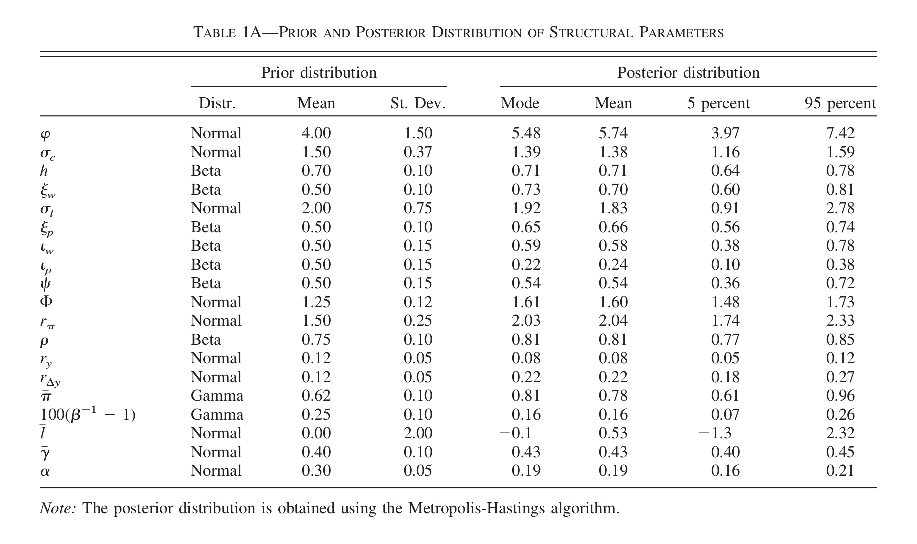
\includegraphics{sw_table1.eps}
   \end{figure} 
\end{frame}
%--------------------------------------

%--------------------------------------
\begin{frame}
  \begin{figure}
    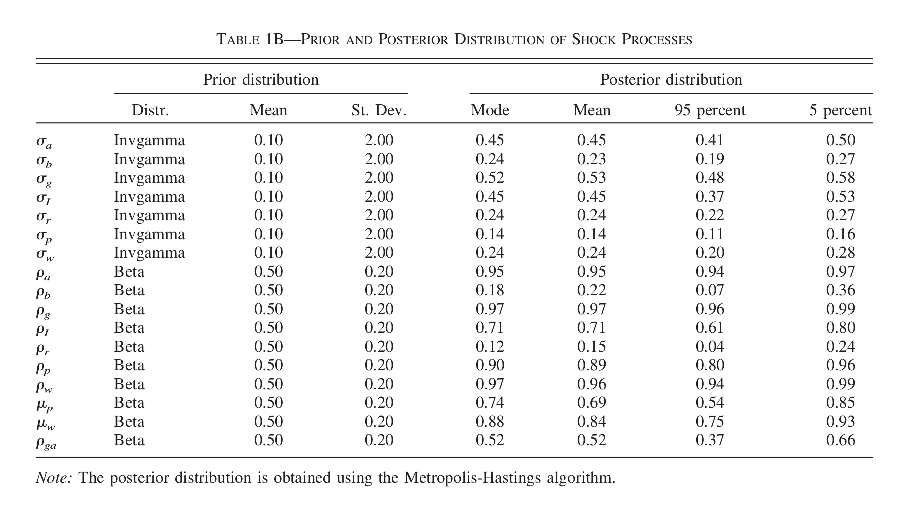
\includegraphics{sw_table1b.eps}
  \end{figure}
\end{frame}
%--------------------------------------

%--------------------------------------
\begin{frame}
  \begin{figure}
    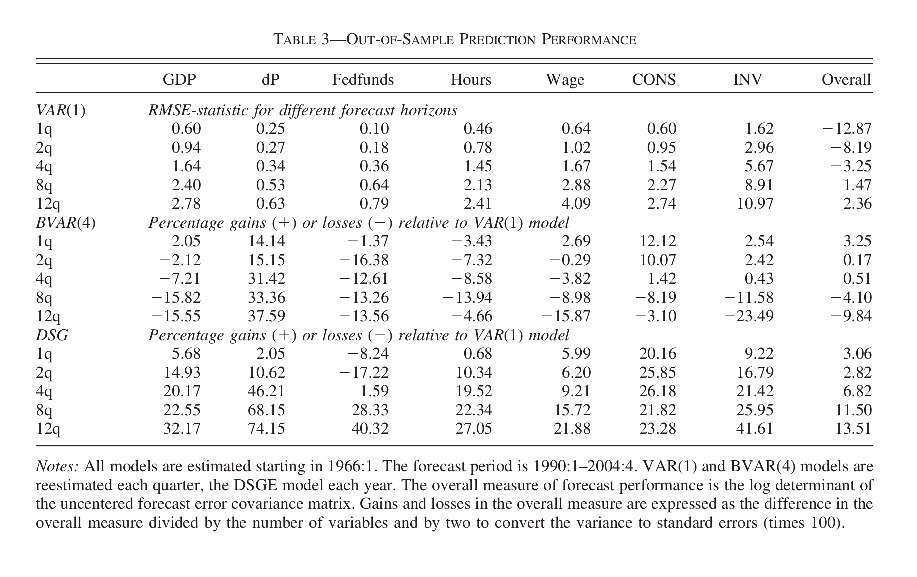
\includegraphics{sw_table3.eps}
  \end{figure}
\end{frame}
%--------------------------------------

%--------------------------------------
\begin{frame}
  \begin{figure}
    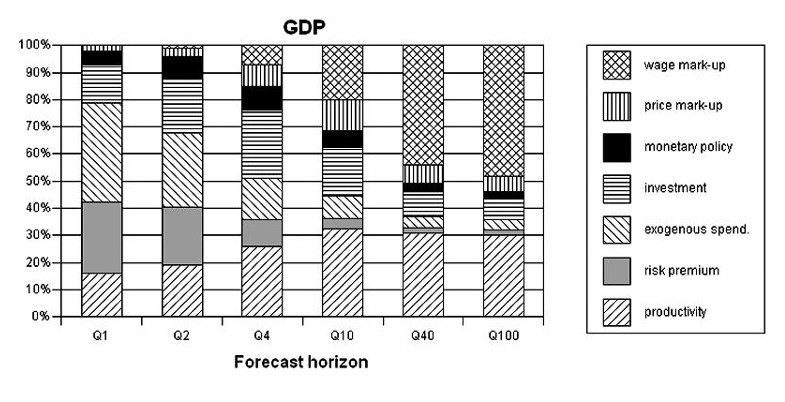
\includegraphics{sw_figure1_gdp.eps}
  \end{figure}
\end{frame}
%--------------------------------------

%--------------------------------------
\begin{frame}
  \begin{figure}
    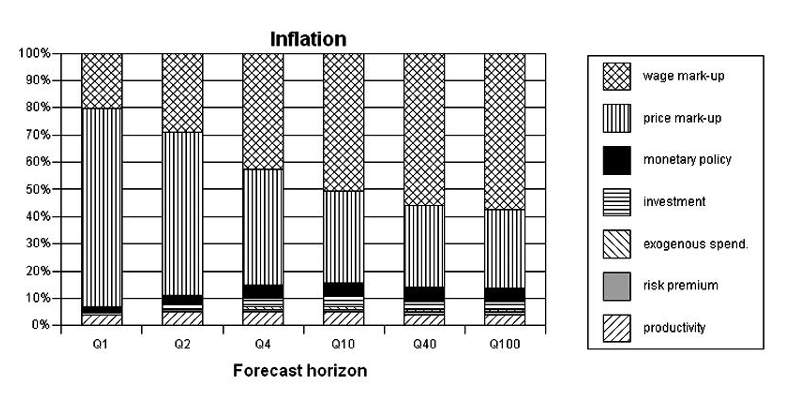
\includegraphics{sw_figure1_inflation.eps}
  \end{figure}
\end{frame}
%--------------------------------------

%--------------------------------------
\begin{frame}
  \begin{figure}
    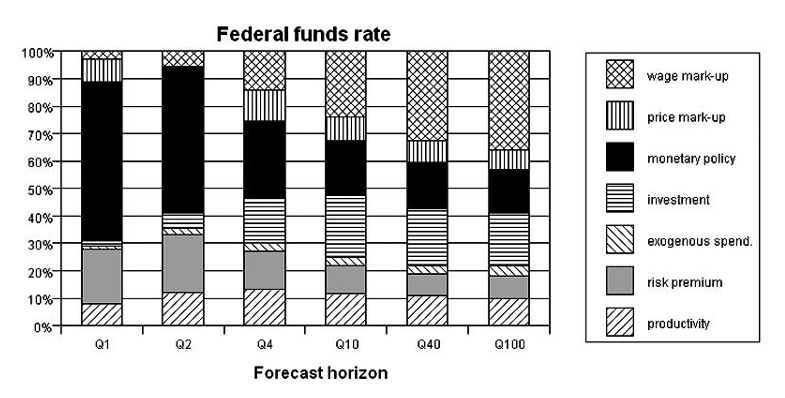
\includegraphics{sw_figure1_interest.eps}
  \end{figure}
\end{frame}
%--------------------------------------

%--------------------------------------
\begin{frame}
  \begin{figure}
    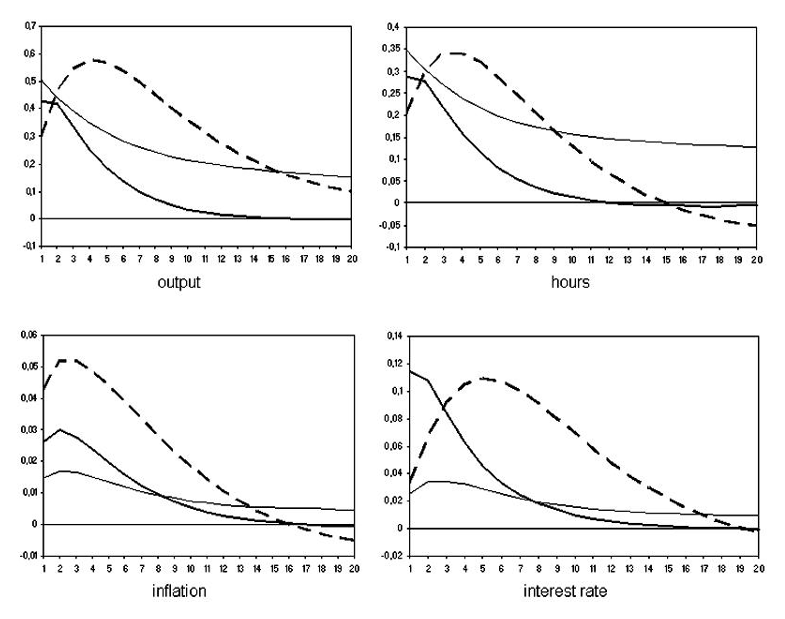
\includegraphics{sw_figure2.eps}
  \end{figure}
\end{frame}
%--------------------------------------

%--------------------------------------
\begin{frame}
  \begin{figure}
    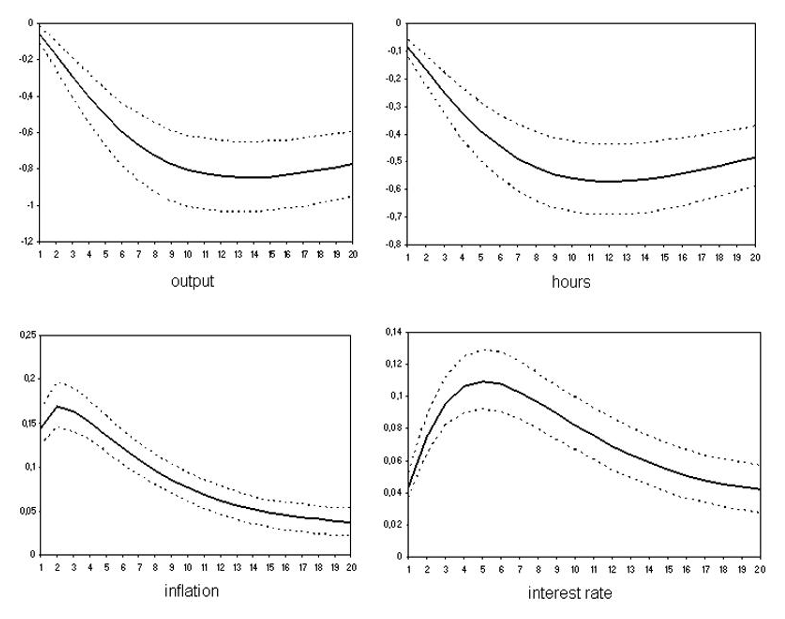
\includegraphics{sw_figure3.eps}
  \end{figure}
\end{frame}
%--------------------------------------

%--------------------------------------
\begin{frame}
  \begin{figure}
    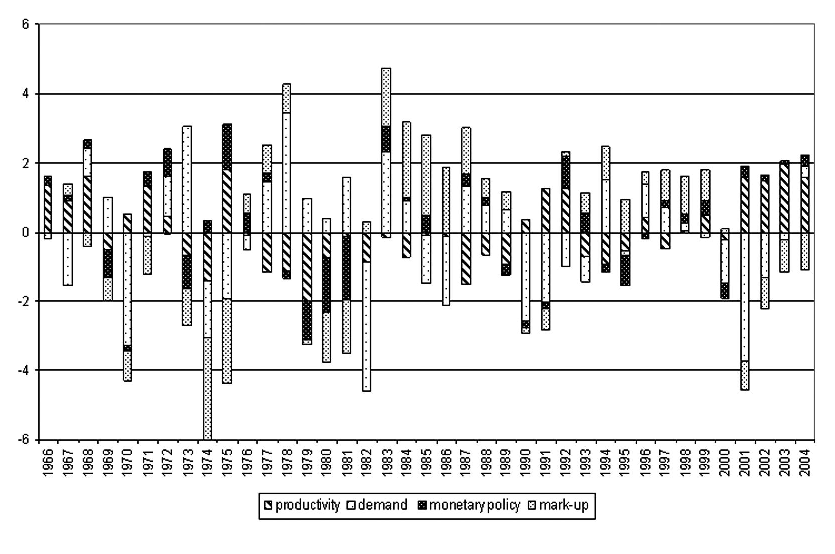
\includegraphics{sw_figure4_gdp.eps}
  \end{figure}
\end{frame}
%--------------------------------------

%--------------------------------------
\begin{frame}
  \begin{figure}
    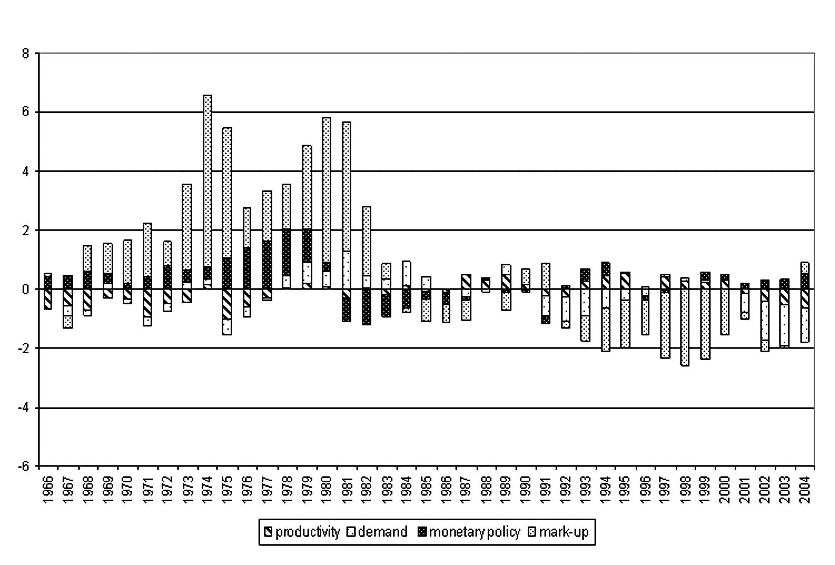
\includegraphics{sw_figure4_inflation.eps}
  \end{figure}
\end{frame}
%--------------------------------------

%--------------------------------------
\begin{frame}
  \begin{figure}
    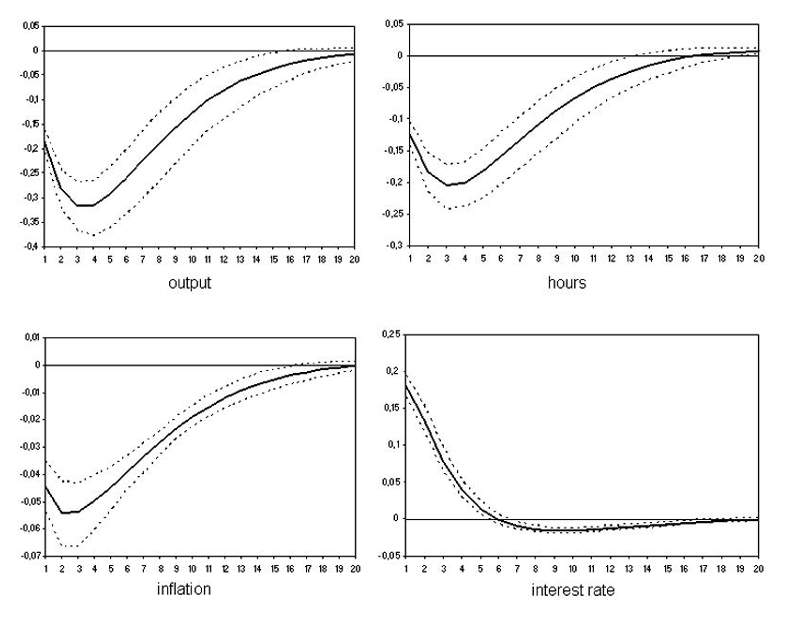
\includegraphics{sw_figure6.eps}
  \end{figure}
\end{frame}
%--------------------------------------


%--------------------------------------
\end{document}
